% Chapter 1

\chapter{理论基础}

\section{恶意代码分类}
恶意代码分类,是当前网络安全领域研究的一个重点。传统基于人工的动态分析和静态分析的研究方法,
存在耗时长,资源开销大的缺点,基于人工智能的自动化恶意代码分类成为新的前沿研究领域,同时也具有很大的应用价值。
这种方法的基本流程如下:
\begin{itemize}
    \item 收集恶意代码样本:首先需要收集大量的恶意代码样本,以便用来训练机器学习模型。
    \item 数据预处理:将恶意代码样本转换为可以输入机器学习模型的数据格式。这通常包括提取恶意代码中的特征,例如文件名、文件大小、代码中使用的API函数等。
    \item 训练机器学习模型:使用恶意代码样本和数据预处理后的数据来训练机器学习模型。常用的机器学习算法包括逻辑回归、支持向量机和决策树等。
    \item 评估机器学习模型:使用测试集对机器学习模型进行评估,测量模型在分类恶意代码方面的准确率。
    \item 应用机器学习模型:将机器学习模型应用到实际的恶意代码分类中,用于快速识别恶意代码的类型。
\end{itemize}

基于机器学习的恶意代码分类方法可以有效地将恶意代码分类为不同的类型,包括病毒、蠕虫、木马、间谍软件等。这对于信息安全来说是非常重要的,因为不同的恶意代码类型具有不同的特征和攻击方式,必须采取不同的防御措施才能有效地保护计算机系统。

\subsection{特征提取}
在实践中,实现基于人工智能的恶意代码分类最重要的就是特征提取,并且将这些特征转化为可以应用于人工智能模型的输入,基本方法如下:\cite{李豪2022恶意代码可视化检测技术研究综述}
\subsubsection{N-gram}
N-gram是一种用于自然语言处理的技术,它可以将文本划分为连续的、相邻的词序列,以便于进行文本分析和处理。

在恶意代码分类方面,基于N-gram的方法可以% Encoding: UTF-8将恶意代码中的代码序列划分为连续的、相邻的代码序列,并利用这些序列的信息来识别恶意代码的类型。

特别的,恶意代码的代码序列中,寄存器的使用一般而言不具备特殊性,所以在进行n-gram的特征提取时,只会单独提取指令代码,而省略指令对象。\cite{Schultz}
\begin{figure}
  \centering
  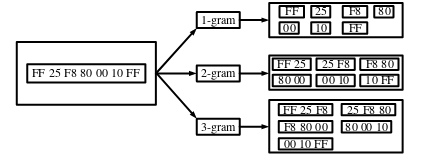
\includegraphics[width=0.7\textwidth]{n-gram.png}
  \caption{N-gram}
  \label{fig:1}
\end{figure}

\subsubsection{灰度图像}
基于灰度图像的恶意代码分类方法是指使用灰度图像来识别恶意代码的类型的方法。灰度图像是一种使用灰度值表示图像的类型,其中灰度值越大,图像的颜色越深。

目前最基本的基于灰度图像的恶意代码检测方法是Nataraj 矢量化:

Nataraj 矢量化将一段二进制代码作为编码源,然后对这一连串二进制代码分组,以8bit表示灰度图像中一个像素点的灰度,从而将一段二进制代码转换为灰度图像。

更进一步的,可以对这个图像通过Steerable Pyramid 将其分割为图像子带,再对其使用GIST作特征提取,将提取到的特征作为人工智能模型的输入。\cite{natarajMalwareImagesVisualization2011}

\subsubsection{彩色图像}
基于彩色图像的恶意代码分类方法是一种用来识别恶意代码的技术。它通过对计算机中的代码进行图像处理来分析其特征,并将其与已知的恶意代码进行比较,以确定其是否具有恶意性。

具体来说,基于彩色图像的恶意代码分类方法首先会将代码转换成图像,然后使用图像处理技术对其进行分析。这些技术可能包括对图像进行颜色分析、纹理分析、边缘检测等。通过对图像进行这些分析,系统可以提取出图像中的特征,并将这些特征与已知的恶意代码进行比较。如果检测到的代码与已知的恶意代码具有较大的相似性,则可以认为该代码具有恶意性。

相较于只含有单个通道灰度图,彩色图像可以保留更多基于相似代码的纹理特征,更容易识别,但是需要的计算量也随之更大。\cite{yiMaliciousCodeDetection2022}

\section{KNN}
KNN(K-Nearest Neighbor, K最近邻算法)是一种分类算法,它的思想是:如果一个样本在特征空间中的k个最相似(即特征空间中最邻近)的样本中的大多数属于某一个类别,则该样本也属于这个类别。KNN算法中,所选择的邻居都是已经正确分类的对象。该方法在定类决策上只依据最邻近的一个或者几个样本的类别来决定待分样本所属的类别。

KNN算法的优点是精度高、对异常值不敏感、无数据输入假定。缺点是计算复杂度高、空间复杂度高。

KNN算法的工作原理如下:
\begin{itemize}
  \item 输入:给定训练数据集和目标变量的取值。
  \item 预处理:对训练数据集进行预处理,并将其转化为可以用于距离计算的数值型数据。
  \item 计算距离:计算待测样本与训练样本之间的距离。
  \item 选择最近邻居:选择距离最小的k个训练样本作为待测样本的最近邻居。
  \item 输出:输出k个最近邻居中出现次数最多的分类结果。
\end{itemize}


在本试验中,输入是由恶意代码转换而来的灰度图片,距离计算采用欧几里德距离。


\section{CNN}

CNN(Convolutional Neural Network, 卷积神经网络)是一种用于图像分类、目标检测和识别等任务的神经网络模型。它的主要思想是利用卷积运算来学习图像的特征,并使用多层神经网络来进行分类。

CNN网络的结构一般包含输入层、卷积层、池化层、全连接层和输出层。输入层用于接收输入图像,卷积层用于学习图像的特征,池化层用于降低图像的尺寸和减少参数,全连接层用于将图像的特征进行分类,输出层用于输出分类结果。

CNN网络的优点是在图像分类任务中表现出色,可以学习到图像的复杂的特征,同时参数少,计算效率高。缺点是对于输入图像的尺寸有要求,训练时间较长。

CNN网络的应用领域很广,比如图像分类、目标检测、图像生成等。它也是目前应用最为广泛的神经网络模型之一。


